\section{Event Receive Packet Processing Module}

The event receiver interface takes events off of the network and
places them on the event bus. They are also placed in a 64-event-deep
FIFO, where they are then sent one event at a time on the Event Bus.

The Event Protocol used to send events to the backplane is the most
complex Soma network protocol, in an attempt to prevent inbound event
overflow. For each inbound event packet (which can contain up to eight
events) we check if there is space in the FIFO; if there is, we commit
it to the internal event FIFO and send a success packet. If there is
insufficient space for all events in the fifo, the entire packet is
aborted and a failure packet is sent back to the originating client.

Inbound event packets are transactional and atomic -- they either
succeed or fail in their entirety.

\subsection{Interface}
The interface for the event receive packet processing module is
straigtforward, with signals to talk to the Event Bus, the TX Mux, and
the Input Control module.

\subsection{Implementation}

\begin{figure}
\begin{centering}
\includegraphics[scale=0.8]{eventreceive.svg}
\end{centering}
\caption{The Network Event Receive interface.}
\label{eventreceive}
\end{figure}

\begin{figure}
\begin{centering}
\includegraphics[scale=0.8]{eventreceive.fsm.svg}
\end{centering}
\caption{The Network Event Receive interface FSM.}
\label{eventreceive.fsm}
\end{figure}

Internally, the Event Receive Packet Processing Module consists of two components:
\begin{itemize}
\item \textbf{Event Bus Output} : this module contains the Event Bus FIFO and is responsible for placing the inbound events onto the Event Bus. 
\item \textbf{Event Response Writer} : this module takes in the packet's header and metadata and returns the success or failure state to the client that originated the packet. 
\end{itemize}

\subsubsection{FSM Steps}

The FSM kicks off with the assertion of the \signal{START} signal,
which enters into a series of states to set the outbound
\signal{INPKTADDR[9:0]} and latch \signal{NONCE}, \signal{DESTMAC},
\signal{DESTPORT}, and \signal{DESTIP}, to allow for us to respond to
the sender.

We next check to see if \signal{ECNT} < \signal{EFREE}; if so, we
start the network event fifo and let it have exclusive access to the
inbound packet buffer while simultaneously starting the event response
writer.

Either the event response writer or the network event fifo can finish
first, so their done signals latch. 

\subsection{Event RX Bus Output FIFO}
\begin{figure}
\begin{centering}
\includegraphics[scale=0.8]{eventreceive.busoutput.svg}
\end{centering}
\caption{The Network Event Receive Bus Output.}
\label{eventreceive.busoutput}
\end{figure}

\begin{figure}
\begin{centering}
\includegraphics[scale=0.8]{eventreceive.busoutput.fsm.svg}
\end{centering}
\caption{The Network Event Receive interface FSM.}
\label{eventreceive.busoutput.fsm}
\end{figure}

The Event RX Bus Output FIFO's addressing scheme assumes that the
first event starts at \signal{ADDROUT[9:0]} = 0, and they are packed
on 16-word boundaries, and they are readable with a single-cycle
latency (a).

On the output side, every ECYCLE we check and see if there is anything
in the FIFO, and if there is, we set up a register set to send it on
the next ECYCLE. 

\subsection{Event Response Writer}

\begin{figure}
\begin{centering}
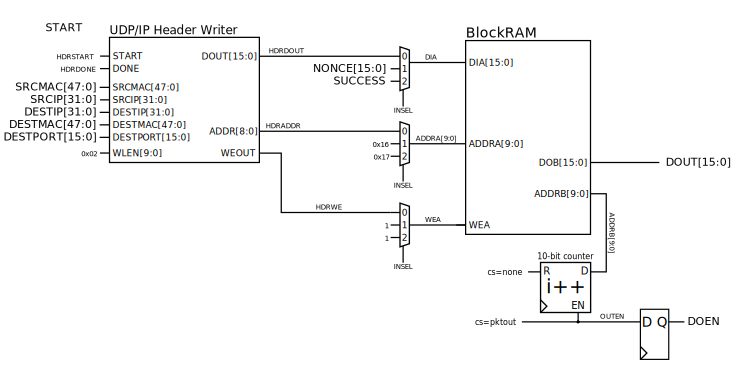
\includegraphics[scale=0.8]{eventreceive.responsewriter.svg}
\end{centering}
\caption{The Network Event Receive Bus Output.}
\label{eventreceive.responsewriter}
\end{figure}

\begin{figure}
\begin{centering}
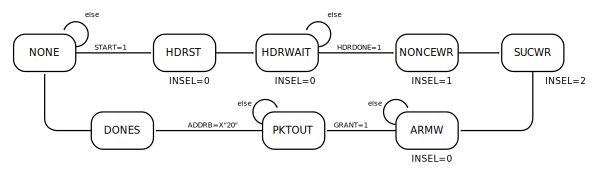
\includegraphics[scale=0.8]{eventreceive.responsewriter.fsm.svg}
\end{centering}
\caption{The Network Event Receive interface FSM.}
\label{eventreceive.responsewriter.fsm}
\end{figure}

The event response writer writes the necessary Ethernet /UDP /IP
header data using the UDP Header Writer module. The nonce and success
state are written to the proper location.

